\documentclass[runningheads]{llncs}
\usepackage[T1]{fontenc}
\usepackage{graphicx}
\usepackage{amsmath}
\usepackage{amssymb}
\usepackage{booktabs}

\newcommand{\method}{\ensuremath{\alpha}\text{-CBM}}

\begin{document}
\title{\method: Label-Free Concept Bottleneck Models for Audio}
\titlerunning{\method}
\author{Amine Maazizi\inst{1,2}\textsuperscript{*} \and
Adam Gassem\inst{1,2}\textsuperscript{*}}
\authorrunning{A. Maazizi and A. Gassem}
\institute{ENSTA Paris, Palaiseau, France \and
MVA, ENS Paris-Saclay, Gif-sur-Yvette, France\\
\email{\{amine.maazizi,adam.gassem\}@ensta.fr}\\
\textsuperscript{*}Equal contribution.}
\maketitle


\begin{abstract}
Concept Bottleneck Models expose interpretable variables but usually require concept annotations. Label-Free CBMs remove this requirement by learning concept projections from multimodal similarity rather than manual concept labels. We introduce \method, an adaptation of Label-Free CBMs to audio that projects task-trained AST features onto CLAP-supervised textual concepts. To better reflect acoustic structure, we augment class-conditioned concepts with dataset-independent perceptual attributes and contrastive dimensions for confusable classes. Across ESC-50, UrbanSound8K, and CREMA-D, broad concepts consistently improve vanilla LF-CBM while retaining competitive classification performance. The resulting bottlenecks are sparse and directly editable for environmental sounds, but denser for speech emotion. Reusing the same bottleneck on overlapping 1-second windows further produces temporal concept trajectories: short-window pooling is weaker than full-clip inference, but reveals when evidence appears and exposes structured failure modes. Audio-specific vocabularies therefore make label-free concept models more useful for sparse, editable, and temporal explanations.
\keywords{Concept bottleneck models \and Audio classification \and Explainable AI \and Temporal explanations}
\end{abstract}

\section{Introduction}
Concept Bottleneck Models (CBMs) expose intervenable variables but conventionally require concept labels~\cite{koh2020concept}. Label-Free CBMs (LF-CBMs) learn concepts from multimodal similarity patterns instead~\cite{oikarinen2023labelfree}. We introduce \method, which transfers LF-CBM to audio using a fine-tuned Audio Spectrogram Transformer (AST)~\cite{gong2021ast} and CLAP supervision~\cite{elizalde2023clap}.

Audio demands modality-specific concepts: events often differ by pitch, harmonicity, roughness, attack, repetition, and reverberation. This raises two questions: which vocabulary best supports a label-free audio bottleneck, and whether a globally trained bottleneck can still provide useful temporal explanations. We therefore augment vanilla LF concepts with broad auditory attributes and contrastive dimensions for confusable classes, evaluate the resulting models on three datasets, and expose exact concept edits and 1-second temporal explanations.

Code, model artifacts, and the interactive demonstration are available at \url{https://github.com/Adam-Ousse/Label-free-CBM-Audio} and \url{https://adam-ousse.github.io/Label-free-CBM-Audio/}, respectively.
\section{Method}
For recording $x_i$ and text concept $c_j$, frozen CLAP encoders provide $p_{ij}=\cos(E_a(x_i),E_t(c_j))$. A linear projection of frozen task-trained AST features and an elastic-net classifier give
\begin{equation}
a_i=W_cf_{\mathrm{AST}}(x_i),\qquad \ell_i=W_F\hat a_i+b_F,
\label{eq:model}
\end{equation}
where $W_c$ matches CLAP activation patterns with the LF-CBM cosine-cubed objective and $\hat a_i$ is standardized on training data. Original LF-CBM filters remove long, class-matching, duplicate, weakly activated, and poorly projected concepts. The language model therefore proposes candidates.

We form $\mathcal C_0=\mathcal C_{\mathrm{LF}}\cup\mathcal C_{\mathrm{broad}}\cup\mathcal C_{\mathrm{contrast}}$. $\mathcal C_{\mathrm{LF}}$ contains class-conditioned audible characteristics. Unlike generic visual attributes, broad acoustic properties can be highly discriminative; thus, dataset-independent $\mathcal C_{\mathrm{broad}}$ captures atomic pitch, spectral, timbral, textural, dynamic, temporal, and spatial properties, generated without class names or semantic events. For $\mathcal C_{\mathrm{contrast}}$, the language model groups acoustically confusable classes and proposes class-name-free dimensions separating each group. We compare LF, LF+broad, LF+contrastive, and their union.

\begin{figure}[t]
\centering
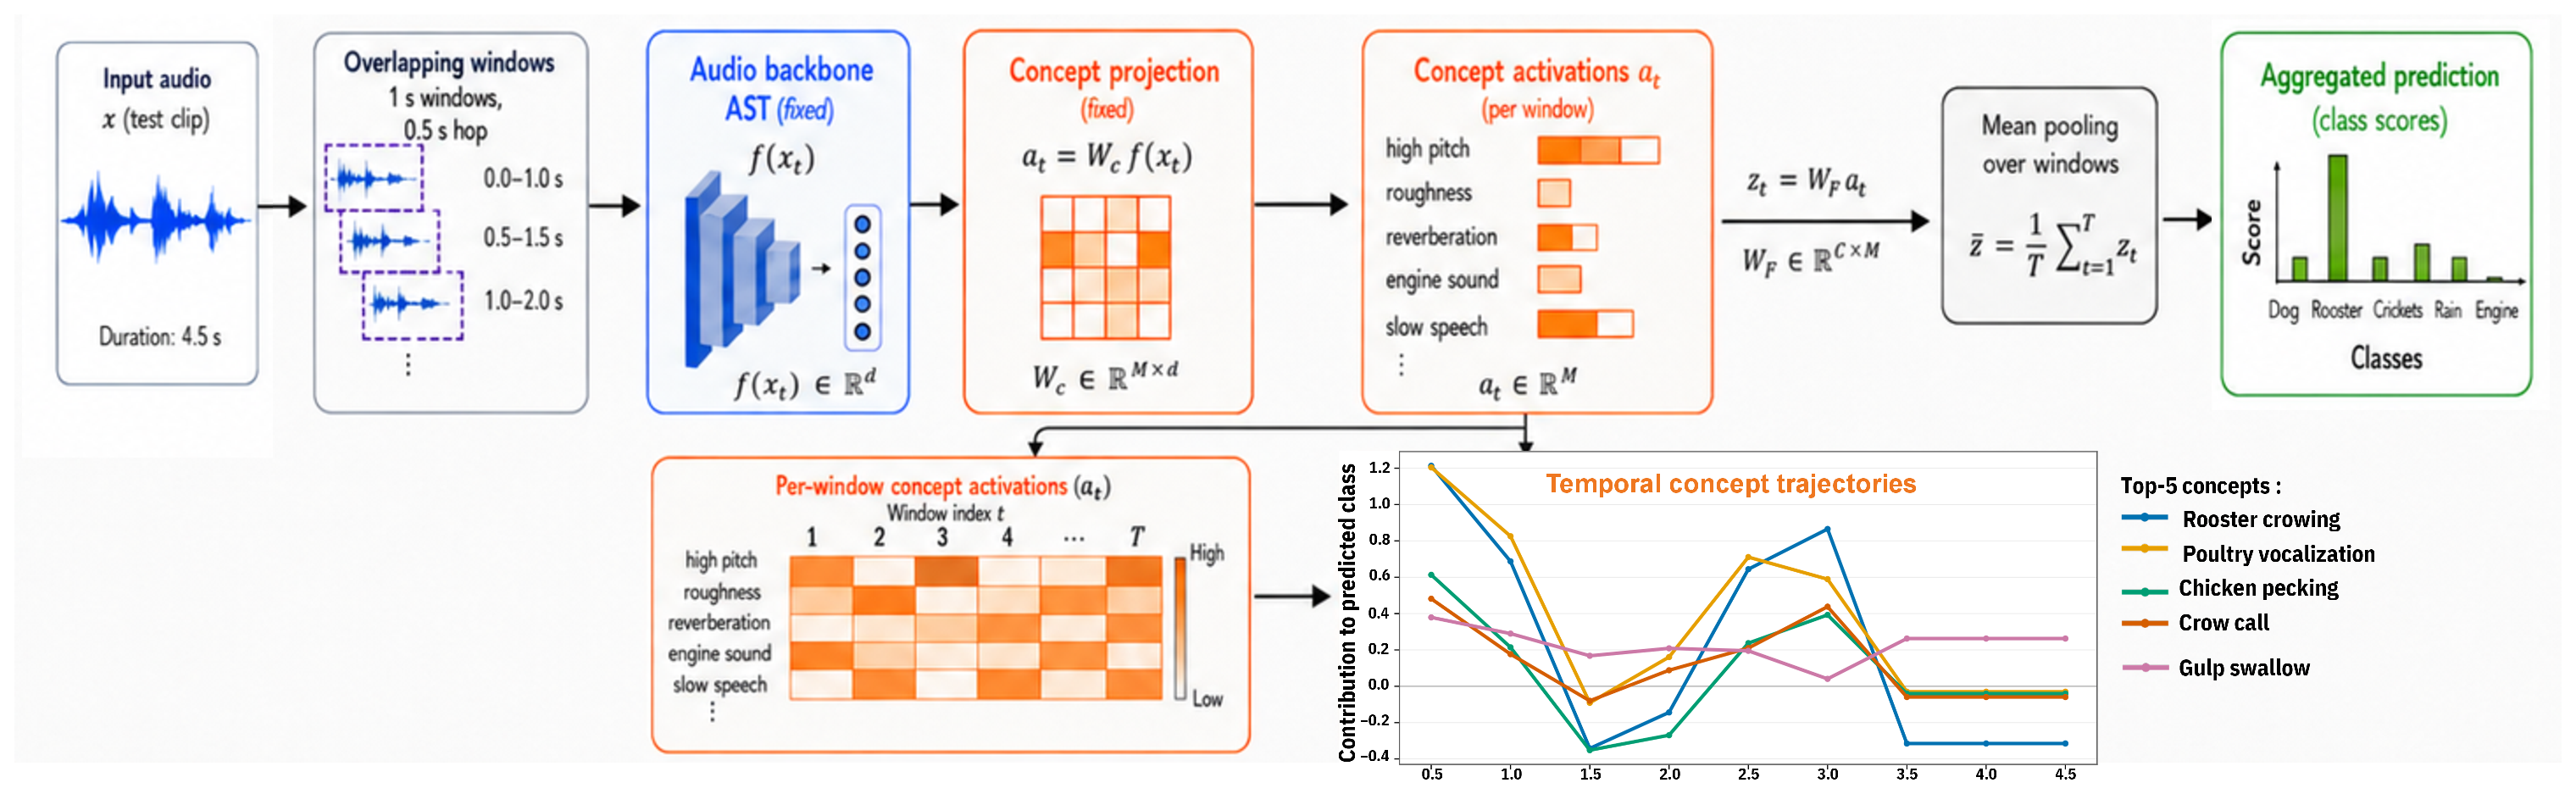
\includegraphics[width=0.92\textwidth]{fig1.eps}
\caption{The CBM reused on overlapping audio windows to obtain time-indexed concept contributions without retraining the global model.} \label{fig1}
\end{figure}

Scaling displayed concept $j$ by $\gamma_j$ changes a logit by $\Delta\ell_k=\sum_{j\in J}(\gamma_j-1)\hat a_jW_{F,kj}$. For temporal explanations, the frozen pipeline processes 1-second windows every 0.5 seconds; $r^{(t)}_{jk}=\hat a^{(t)}_jW_{F,kj}$ localizes concept evidence. Mean, max, and log-mean-exp pooling form the segmented-inference ablation; full-clip logits remain primary.

\section{Experiments and Results}
The train/validation/test sizes are 1,200/400/400 for ESC-50~\cite{piczak2015esc}, 7,079/816/837 for UrbanSound8K folds 1--8/9/10~\cite{salamon2014urbansound}, and 5,357/596/1,489 for CREMA-D~\cite{cao2014cremad}. Fine-tuned AST checkpoints serve as baselines and feature extractors. We report accuracy, macro-F1, and sparse-head zero weights ($|W_{F,kj}|\leq10^{-5}$). Variants share the split, AST features, projection and classifier settings, and differ only in candidate vocabulary. Results use one fixed split and seed; small differences are not claimed significant.

\begin{table}[t]
\caption{Fixed-split test results (\%). ``Kept/in.'' is the post-filter concept count; ``Sp.'' is head sparsity. Bold marks the best CBM macro-F1. CREMA-D uses the latest targeted rerun.}
\label{tab:results}
\centering
\footnotesize
\setlength{\tabcolsep}{2.7pt}
\renewcommand{\arraystretch}{0.90}
\begin{tabular}{@{}llrrrr@{}}
\toprule
Dataset & Model & Acc. & F1 & Kept/in. & Sp. \\
\midrule
ESC-50 & AST & 93.50 & 93.28 & -- & -- \\
 & LF & 93.00 & 92.97 & 596/603 & 91.78 \\
 & LF + broad & \textbf{93.50} & \textbf{93.39} & 671/683 & 92.58 \\
 & LF + contrastive & 93.25 & 93.01 & 689/700 & 92.82 \\
 & Full union & 92.75 & 92.70 & 761/777 & 93.13 \\
\midrule
UrbanSound8K & AST & 89.01 & 90.03 & -- & -- \\
 & LF & 89.37 & 90.60 & 133/140 & 81.88 \\
 & LF + broad & \textbf{89.84} & \textbf{90.94} & 212/224 & 86.04 \\
 & LF + contrastive & 89.73 & 90.76 & 178/185 & 86.07 \\
 & Full union & 89.84 & 90.78 & 255/269 & 87.69 \\
\midrule
CREMA-D (targeted) & AST & 70.05 & 52.76 & -- & -- \\
 & LF & 69.44 & 50.65 & 311/399 & 88.00 \\
 & LF + broad & 69.78 & 50.69 & 481/598 & 91.34 \\
 & LF + contrastive & 69.51 & 49.86 & 396/506 & 90.07 \\
 & Full union & \textbf{70.25} & \textbf{51.58} & 548/701 & 92.79 \\
\bottomrule
\end{tabular}
\end{table}

Broad concepts improve vanilla LF-CBM by 0.50 and 0.48 accuracy points on ESC-50 and UrbanSound8K, respectively, and give the best CBM macro-F1 on both datasets (Table~\ref{tab:results}). LF+broad matches AST accuracy on ESC-50 and improves UrbanSound8K accuracy/macro-F1 by 0.84/0.91 points. In the latest targeted CREMA-D rerun, the full union reaches 70.25/51.58, exceeding AST accuracy by 0.20 points while remaining 1.18 macro-F1 points below it. Its prompt design followed inspection of earlier errors, so this result should be interpreted as a diagnostic follow-up rather than an untouched benchmark. The targeted source ablation shows that the full union improves targeted LF by 0.80/0.93 points in accuracy/macro-F1.

Targeted edits to concept activations can alter model predictions, demonstrating direct intervention through the bottleneck. Temporal trajectories further localize interpretable evidence, for example exposing \emph{giggling} behind a crying-baby$\rightarrow$laughing error. Mean-pooled segmented LF+broad inference reaches 81.75/81.86, 83.63/83.02, and 59.17/23.80 accuracy/macro-F1 on ESC-50, UrbanSound8K, and CREMA-D, respectively, remaining below full-clip inference. Short windows therefore serve primarily as a diagnostic view of \emph{when} concepts support a prediction rather than as a stronger classifier. The targeted CREMA-D source ablation is reported in Table~\ref{tab:results}; its vocabulary was designed after inspecting initial failures.


\section{Conclusion}
\method{} enables editable audio predictions through automatically constructed concepts. Broad perceptual concepts improve vanilla LF-CBM and yield sparse, competitive environmental-sound models. The latest targeted speech-specific vocabulary reaches competitive CREMA-D accuracy, while its remaining macro-F1 gap and the fixed-split, speaker-overlapping protocol expose limitations for emotional prosody. One-second inference localizes concept evidence in time but complements rather than replaces full-clip prediction.

\bibliographystyle{splncs04}
\bibliography{references}
\end{document}
